\begin{exercice*}[Des \oe ufs biologiques]
    Francis veut se lancer dans la production d'\oe ufs biologiques. Son terrain est rectangulaire.
    Il fait $110$ m de long sur $30$ m de large. Il va séparer ce terrain en deux parties rectangulaires :
    \begin{itemize}
        \item Une partie \og Couverte \fg.
        \item Une partie \og Plein air \fg.
    \end{itemize}
    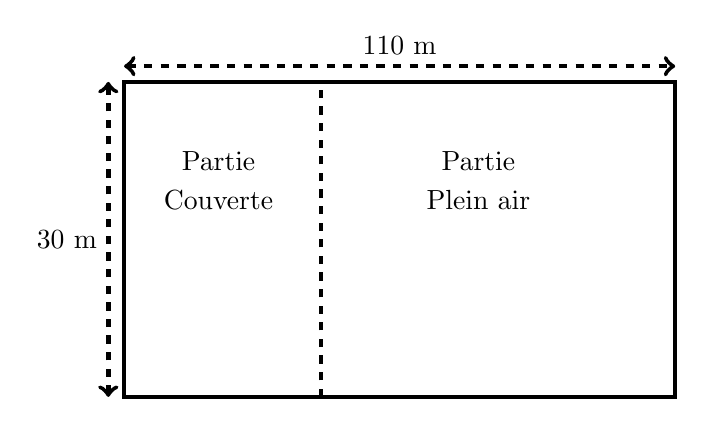
\begin{tikzpicture}
        % \draw[help lines, color=gray!30, dashed] (0,0) grid (9,6);
        \draw[color=black, ultra thick] (1,1) rectangle ++(7,4);        
        \draw[<->,dashed, ultra thick] (1,5.2)--(8,5.2);
        \draw[shift={(4.5,5.2)},color=black,ultra thick] node[above,fill=white] {$110$ m};
        \draw[<->,dashed, ultra thick] (.8,1)--(0.8,5);
        \draw[shift={(0.8,3)},color=black,ultra thick] node[left,fill=white] {$30$ m};
        \draw[-,dashed, ultra thick] (3.5,1)--(3.5,5);
        \draw[shift={(2.2,4)},color=black,ultra thick] node[midway,fill=white] {Partie};
        \draw[shift={(2.2,3.5)},color=black,ultra thick] node[midway,fill=white] {\og Couverte \fg};
        \draw[shift={(5.5,4)},color=black,ultra thick] node[midway,fill=white] {Partie};
        \draw[shift={(5.5,3.5)},color=black,ultra thick] node[midway,fill=white] {\og Plein air \fg};
    \end{tikzpicture}

    Pour avoir la qualitifcation \og biologique \fg, Francis a l'obligation
    de respecter les règles ci-dessous.
    
    \begin{tabularx}{0.48\textwidth}{|C|C|}
        \hline
        \textbf{Patie \og Couverte \fg} & \textbf{Partie \og Plein air \fg} \tabularnewline
        utilisée pour toutes les poules quand il fait nuit        
        & 
        utilisée pour toutes les poules quand il fait jour \tabularnewline
        \hline
        $6$ poules maximum \\par m\up{$2$} & $4$ m\up{$2$} minimum \\par poule\tabularnewline
        \hline
    \end{tabularx}    

      \textit{(Src : Institut Technologique de l'Agriculture Biologique)}

      Il a prévu que la partie couverte ait une surface \\ de $150$ m\up{$2$}.
      \begin{enumerate}
        \item Montre que l'aire de la partie \og Plein air \fg \\est de $\num{3150}$ m\up{$2$}.
        \item Peut-il élever $800$ poules dans son installation ?
        \item Combien de poules au maximum pourrait-il élever dans installation ?
       \end{enumerate}
\end{exercice*}
\begin{corrige}
    %\setcounter{partie}{0} % Pour s'assurer que le compteur de \partie est à zéro dans les corrigés
    \phantom{rrr}    
    \begin{multicols}2
        \begin{enumerate}
            \item .
            \item .
        \end{enumerate}
    \end{multicols}
\end{corrige}

